
\chapter{Aftellen van IPv4}
\label{ch:h4}

Dit hoofdstuk bespreekt wat de uitputting van IPv4 juist inhoudt, hoe deze tot zover is kunnen komen en wat een oplossing is om hiermee om te gaan. Ook zal er visueel aangetoond worden hoe we er vandaag de dag tegenover staan en wat er de komende maanden zal gebeuren rond IPv4 uitputting en IPv6.

Op 3 februari 2011 had IANA (Internet Assigned numbers Authority) aangekondigd dat hun vrije IPv4 pool volledig uitgeput was. De IPv4 uitputting betekent niet dat het einde van het internet is aangebroken. Deze term wordt gebruikt om aan te tonen dat er geen niet-toegewezen IPv4 adressen beschikbaar zijn om uit te delen. Door de grote groei aan IoT, mobiele apparaten en andere geconnecteerde apparaten zijn de beschikbare adressen op een zeer snelle en korte tijd uitgedeeld. Dit werd nooit verwacht tijdens de bouw van IPv4 en werd ook niet gemaakt om heel de wereld in contact te brengen met het internet. Als gevolg was er dus het IPv6 protocol ontwikkeld die de uitputting van IPv4 zou wegnemen.

RIPE NCC, die verantwoordelijk is voor Europa, is begonnen op 14 september 2012 met het uitdelen van zijn laatste /8 blok. De /8 blok bevat de laatste beschikbare IPv4 adressen om uit te delen en bevat 16777216 (2 tot de 24) adressen. Volgens de policy van RIPE NCC is het voor de leden enkel mogelijk om een /22 (1024 adressen) blok aan te vragen, ook al kunnen ze grondig aantonen dat er een grotere blok nodig is krijgen ze maar een /22. Ook zal er geen nieuwe PI (Provider Independent) aangesteld worden.

Voor het bereiken van de laatste /8 blok zijn er verschillende fases ondernomen. Fase 0 was het uitdelen van de IPv4 adressen. Op dat moment was er nog geen sprake van een totale uitputting. Tijdens deze fase werden adressen enkel toegewezen als de evaluatie ook volledig afgerond was. Er werden dus ook geen adressen gereserveerd of aan de kant gehouden tijdens deze evaluatie. Verzoeken naar adressen werden grondig gecontroleerd door een IPRA (IP resource Analyst) en voerde interne controle uit \autocite{RIPE2016Fases}.

Het bereiken van fase 1 vond plaats op 4 september 2012. Deze fase werd geactiveerd als er een kritieke toestand plaats vond bij de beschikbare adressen. Op dit moment was er nog een voorraad van één maand of één /10 blok naast /8 om uit te delen. Verder werden de controles zwaarder en grondiger behandeld \autocite{RIPE2016Fases}.

Momenteel situeren we onszelf in fase 2. Deze fase ging van start op 14 september 2012, enkele dagen nadat fase 1 werd bereikt. Bij het begin van deze fase werden alle verzoeken die in de wachtrij stonden bevroren. Zij werden op de hoogte gebracht dat de laatste /8 blok en werd ingezet en verdeeld. Enkel de LIRs die in aamerking komen zullen eenmalig een /22 toegewezen krijgen \autocite{RIPE2016Fases}.

Op 10 april 2018 waren er nog 0.12 miljoen adressen over of 0.01 /8s. Vandaag zijn er geen beschikbare adressen meer over in de blok, dit werd bereikt vanaf 17 april 2018. Nu de laatste blok volledig op is wil dit niet zeggen dat er geen beschikbare adressen meer over zijn. RIPE NCC is momenteel bezig met het herstellen van andere adressen. Deze kunnen gaan van het terugnemen van adressen als een bepaalde LIR is gestopt en van gerecupereerde adressen van IANA’s pool. Maar vooraleer deze adressen worden uitgedeeld en toegewezen blijven ze in quarantaine. Momenteel is er ook geen exacte datum of tijdstip vastgelegd wanneer adressen uit de quarantaine worden gehaald klaar om uitgedeeld te worden  \autocite{RIPE2014}. 

\begin{figure}
\centering
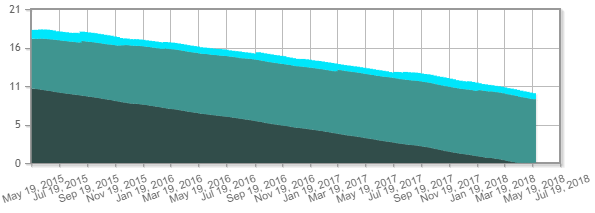
\includegraphics[width=\textwidth,height=\textheight,keepaspectratio]{exhaustion1.PNG}
\caption{IPv4 uitputting \autocite{RIPE2014}}
\end{figure}

Deze grafiek geeft een evolutie aan van beschikbare IPv4 adressen. In bovenstaande grafiek is er duidelijk te zien dat naar gelang de tijd de beschikbare adressen dalen. De donkere kleur staat voor de laatste /8 blok die vrijgegeven is. De licht groene kleur heeft dan meer een stijgende evolutie gekend. Dit zijn de adressen die gerecupereerd zijn van IANA en van LIRs die gestopt zijn. In dit deel komen er dus meer adressen vrij maar blijven ze wel in quarantaine. de blauwe kleur bovenaan toont de gereserveerde adressen aan. Deze worden ingedeeld in een /13 voor tijdelijke toewijzingen, /16 voor IXPs (Internet Exchange Point) en nog een /16 voor onvoorziene omstandigheden die kunnen plaatsvinden. Ook hierin zitten enkele gerecupereerde adressen in quarantaine  \autocite{RIPE2014}.

Op 8 mei 2018 zijn er in totaal nog 9.70 miljoen adressen over waarvan er maar 8.89 miljoen ter beschikking zijn. Zoals we al eerder vernomen hadden, is het aantal in de laatste 185 /8 blok enorm klein. Het aantal beschikbare adressen staat op 0.04 miljoen adressen. Al de gerecupereerde adressen komen samen neer op een 8.85 miljoen adressen. Maar deze zijn dus nog steeds in quarantaine en komen nog niet vrij. De gereserveerde adressen zijn niet beschikbaar en tellen mee voor 0.81 miljoen \autocite{RIPE2014}.

\begin{figure}
\centering
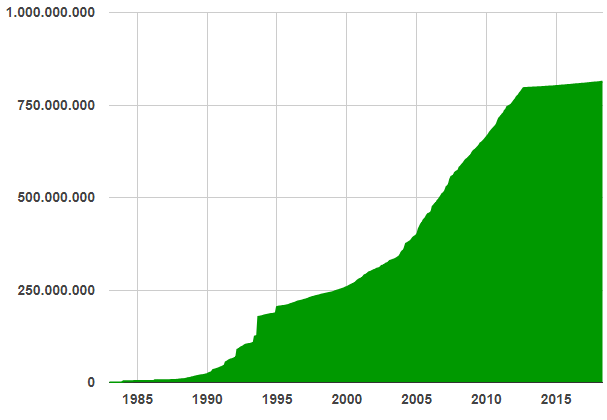
\includegraphics[width=\textwidth,height=\textheight,keepaspectratio]{exhaustion2.PNG}
\caption{IPv4 evolutie \autocite{RIR2018}}
\end{figure}

De grafiek hierboven toont de evolutie van IPv4 in de RIPE NCC zone, ook wel verantwoordelijke voor Europa. De groei dat er is gekomen vanaf de jaren 2000 is immens. Als we verder kijken naar het jaartal 2012, wanneer de laatste 185 /8 blok was aangekondigd, zien we een sterke verandering in de groei. De groei die het tussen het jaar 2012 en heden heeft een zeer kleine stijgingsfactor. Dit komt voornamelijk door de policies die zijn opgesteld door RIPE om met de laatst beschikbare blok voorzichtig overweg te gaan. Hierbij werd er grondig gekeken en in kleinere maten adressen toegewezen waardoor ze zo lang mogelijk de volledige uitputting wilden tegengaan.

\section{Besluit}

Enkele conclusies die er kunnen gemaakt worden zijn, dat komende maanden een hoogtepunt zullen zijn voor zowel IPv4 als voor IPv6. Voor IPv4 kan dit het volledig einde betekenen van de blok wat voor IPv6 een goede zaak kan betekenen. Nu het moeilijker is om nog een range van IPv4 adressen te krijgen gaat er meer overschakelen naar een IPv6 range. Hierdoor zal de vraag naar IPv6 stijgen en de ontwikkeling en overgang sneller in gang gezet worden.  